\documentclass[twoside]{book}

% Packages required by doxygen
\usepackage{fixltx2e}
\usepackage{calc}
\usepackage{doxygen}
\usepackage[export]{adjustbox} % also loads graphicx
\usepackage{graphicx}
\usepackage[utf8]{inputenc}
\usepackage{makeidx}
\usepackage{multicol}
\usepackage{multirow}
\PassOptionsToPackage{warn}{textcomp}
\usepackage{textcomp}
\usepackage[nointegrals]{wasysym}
\usepackage[table]{xcolor}

% Font selection
\usepackage[T1]{fontenc}
\usepackage[scaled=.90]{helvet}
\usepackage{courier}
\usepackage{amssymb}
\usepackage{sectsty}
\renewcommand{\familydefault}{\sfdefault}
\allsectionsfont{%
  \fontseries{bc}\selectfont%
  \color{darkgray}%
}
\renewcommand{\DoxyLabelFont}{%
  \fontseries{bc}\selectfont%
  \color{darkgray}%
}
\newcommand{\+}{\discretionary{\mbox{\scriptsize$\hookleftarrow$}}{}{}}

% Page & text layout
\usepackage{geometry}
\geometry{%
  a4paper,%
  top=2.5cm,%
  bottom=2.5cm,%
  left=2.5cm,%
  right=2.5cm%
}
\tolerance=750
\hfuzz=15pt
\hbadness=750
\setlength{\emergencystretch}{15pt}
\setlength{\parindent}{0cm}
\setlength{\parskip}{3ex plus 2ex minus 2ex}
\makeatletter
\renewcommand{\paragraph}{%
  \@startsection{paragraph}{4}{0ex}{-1.0ex}{1.0ex}{%
    \normalfont\normalsize\bfseries\SS@parafont%
  }%
}
\renewcommand{\subparagraph}{%
  \@startsection{subparagraph}{5}{0ex}{-1.0ex}{1.0ex}{%
    \normalfont\normalsize\bfseries\SS@subparafont%
  }%
}
\makeatother

% Headers & footers
\usepackage{fancyhdr}
\pagestyle{fancyplain}
\fancyhead[LE]{\fancyplain{}{\bfseries\thepage}}
\fancyhead[CE]{\fancyplain{}{}}
\fancyhead[RE]{\fancyplain{}{\bfseries\leftmark}}
\fancyhead[LO]{\fancyplain{}{\bfseries\rightmark}}
\fancyhead[CO]{\fancyplain{}{}}
\fancyhead[RO]{\fancyplain{}{\bfseries\thepage}}
\fancyfoot[LE]{\fancyplain{}{}}
\fancyfoot[CE]{\fancyplain{}{}}
\fancyfoot[RE]{\fancyplain{}{\bfseries\scriptsize Generated by Doxygen }}
\fancyfoot[LO]{\fancyplain{}{\bfseries\scriptsize Generated by Doxygen }}
\fancyfoot[CO]{\fancyplain{}{}}
\fancyfoot[RO]{\fancyplain{}{}}
\renewcommand{\footrulewidth}{0.4pt}
\renewcommand{\chaptermark}[1]{%
  \markboth{#1}{}%
}
\renewcommand{\sectionmark}[1]{%
  \markright{\thesection\ #1}%
}

% Indices & bibliography
\usepackage{natbib}
\usepackage[titles]{tocloft}
\setcounter{tocdepth}{3}
\setcounter{secnumdepth}{5}
\makeindex

% Hyperlinks (required, but should be loaded last)
\usepackage{ifpdf}
\ifpdf
  \usepackage[pdftex,pagebackref=true]{hyperref}
\else
  \usepackage[ps2pdf,pagebackref=true]{hyperref}
\fi
\hypersetup{%
  colorlinks=true,%
  linkcolor=blue,%
  citecolor=blue,%
  unicode%
}

% Custom commands
\newcommand{\clearemptydoublepage}{%
  \newpage{\pagestyle{empty}\cleardoublepage}%
}

\usepackage{caption}
\captionsetup{labelsep=space,justification=centering,font={bf},singlelinecheck=off,skip=4pt,position=top}

%===== C O N T E N T S =====

\begin{document}

% Titlepage & ToC
\hypersetup{pageanchor=false,
             bookmarksnumbered=true,
             pdfencoding=unicode
            }
\pagenumbering{alph}
\begin{titlepage}
\vspace*{7cm}
\begin{center}%
{\Large Assignment1\+Part4\+Dice }\\
\vspace*{1cm}
{\large Generated by Doxygen 1.8.12}\\
\end{center}
\end{titlepage}
\clearemptydoublepage
\pagenumbering{roman}
\tableofcontents
\clearemptydoublepage
\pagenumbering{arabic}
\hypersetup{pageanchor=true}

%--- Begin generated contents ---
\chapter{Class Index}
\section{Class List}
Here are the classes, structs, unions and interfaces with brief descriptions\+:\begin{DoxyCompactList}
\item\contentsline{section}{\hyperlink{class_dice}{Dice} }{\pageref{class_dice}}{}
\end{DoxyCompactList}

\chapter{File Index}
\section{File List}
Here is a list of all documented files with brief descriptions\+:\begin{DoxyCompactList}
\item\contentsline{section}{\hyperlink{_dice_8cpp}{Dice.\+cpp} \\*Definition of a \hyperlink{class_dice}{Dice}, from d20 game }{\pageref{_dice_8cpp}}{}
\item\contentsline{section}{\hyperlink{_dice_8h}{Dice.\+h} \\*Define \hyperlink{class_dice}{Dice} Class }{\pageref{_dice_8h}}{}
\item\contentsline{section}{\hyperlink{_dice_exceptions_8h}{Dice\+Exceptions.\+h} \\*Definition of some of dice exceptions }{\pageref{_dice_exceptions_8h}}{}
\item\contentsline{section}{\hyperlink{_dice_roller_8cpp}{Dice\+Roller.\+cpp} \\*The \hyperlink{class_dice}{Dice} Roller is taking a rule from the user, and execute this rule, by setting up dice, and rolling them all }{\pageref{_dice_roller_8cpp}}{}
\item\contentsline{section}{\hyperlink{_dice_roller_8h}{Dice\+Roller.\+h} \\*Define class of Class\+Roller }{\pageref{_dice_roller_8h}}{}
\item\contentsline{section}{\hyperlink{_run_app_8cpp}{Run\+App.\+cpp} \\*Run unit test, and main program. (Driver) }{\pageref{_run_app_8cpp}}{}
\item\contentsline{section}{\hyperlink{_test_dice_8cpp}{Test\+Dice.\+cpp} \\*Define test cases to test the \hyperlink{class_dice_roller}{Dice\+Roller} }{\pageref{_test_dice_8cpp}}{}
\item\contentsline{section}{\hyperlink{_test_dice_8h}{Test\+Dice.\+h} \\*Definition of class to test the \hyperlink{class_dice}{Dice} }{\pageref{_test_dice_8h}}{}
\end{DoxyCompactList}

\chapter{Class Documentation}
\hypertarget{class_dice}{}\section{Dice Class Reference}
\label{class_dice}\index{Dice@{Dice}}


{\ttfamily \#include \char`\"{}Dice.\+h\char`\"{}}

\subsection*{Public Member Functions}
\begin{DoxyCompactItemize}
\item 
\hyperlink{class_dice_a6b9eadd945ad8fd3840379c8824e5d48_a6b9eadd945ad8fd3840379c8824e5d48}{Dice} ()
\end{DoxyCompactItemize}
\subsection*{Static Public Member Functions}
\begin{DoxyCompactItemize}
\item 
static int \hyperlink{class_dice_a4ca42849612d2c9182f1d93deaa4cfb1_a4ca42849612d2c9182f1d93deaa4cfb1}{roll} (const string \&Expr)
\end{DoxyCompactItemize}
\subsection*{Static Private Member Functions}
\begin{DoxyCompactItemize}
\item 
static bool \hyperlink{class_dice_a7fb1c52019fa79aa3b73e6610da9139c_a7fb1c52019fa79aa3b73e6610da9139c}{parse} (const string \&Expr, int \&dice\+Number, int \&dice\+Kind, int \&addition)
\end{DoxyCompactItemize}
\subsection*{Static Private Attributes}
\begin{DoxyCompactItemize}
\item 
static const int \hyperlink{class_dice_afb857d94c4abede11939a308770ea72b_afb857d94c4abede11939a308770ea72b}{D\+I\+C\+E\+K\+I\+ND} = 7
\item 
static const int \hyperlink{class_dice_a0a00c7ba6e7486d9cbcf7c8c64c65b1a_a0a00c7ba6e7486d9cbcf7c8c64c65b1a}{D\+I\+C\+E\+N\+UM} \mbox{[}\hyperlink{class_dice_afb857d94c4abede11939a308770ea72b_afb857d94c4abede11939a308770ea72b}{D\+I\+C\+E\+K\+I\+ND}\mbox{]} = \{ 4, 6, 8, 10, 12, 20, 100 \}
\end{DoxyCompactItemize}


\subsection{Detailed Description}
include \char`\"{}\+Dice.\+h\char`\"{} this is included as it is where we created and specificed the \hyperlink{class_dice}{Dice} Class include \char`\"{}stdlib.\+h\char`\"{} This Library includes several marcos, functions, and variable types needed, such as the N\+U\+LL macro, and the rand function include \char`\"{}iosstream\char`\"{} This library includes basic input and output services such as \char`\"{}cout\char`\"{} in this case include \char`\"{}time.\+h\char`\"{} This library includes the variables and functions used to start the projects random number generator using srand(time) 

\subsection{Constructor \& Destructor Documentation}
\hypertarget{class_dice_a6b9eadd945ad8fd3840379c8824e5d48_a6b9eadd945ad8fd3840379c8824e5d48}{}\label{class_dice_a6b9eadd945ad8fd3840379c8824e5d48_a6b9eadd945ad8fd3840379c8824e5d48} 
\index{Dice@{Dice}!Dice@{Dice}}
\index{Dice@{Dice}!Dice@{Dice}}
\subsubsection{\texorpdfstring{Dice()}{Dice()}}
{\footnotesize\ttfamily Dice\+::\+Dice (\begin{DoxyParamCaption}{ }\end{DoxyParamCaption})}

include \char`\"{}\+Dice.\+h\char`\"{} this is included as it is where we created and specificed the \hyperlink{class_dice}{Dice} Class include \char`\"{}stdlib.\+h\char`\"{} This Library includes several marcos, functions, and variable types needed, such as the N\+U\+LL macro, and the rand function include \char`\"{}iosstream\char`\"{} This library includes basic input and output services such as \char`\"{}cout\char`\"{} in this case include \char`\"{}time.\+h\char`\"{} This library includes the variables and functions used to start the projects random number generator using srand(time) This starts the random number generator

\subsection{Member Function Documentation}
\hypertarget{class_dice_a7fb1c52019fa79aa3b73e6610da9139c_a7fb1c52019fa79aa3b73e6610da9139c}{}\label{class_dice_a7fb1c52019fa79aa3b73e6610da9139c_a7fb1c52019fa79aa3b73e6610da9139c} 
\index{Dice@{Dice}!parse@{parse}}
\index{parse@{parse}!Dice@{Dice}}
\subsubsection{\texorpdfstring{parse()}{parse()}}
{\footnotesize\ttfamily bool Dice\+::parse (\begin{DoxyParamCaption}\item[{const string \&}]{Expr,  }\item[{int \&}]{dice\+Number,  }\item[{int \&}]{dice\+Kind,  }\item[{int \&}]{addition }\end{DoxyParamCaption})\hspace{0.3cm}{\ttfamily [static]}, {\ttfamily [private]}}

parses the expression given to us Expr\+: expression provided is xdy\mbox{[}+z\mbox{]} dice\+Number\+: the x value gets saved here dice\+Type\+: the y value gets saved here addition\+: the z value gets saved here if it is specified, otherwise it is set to 0 returns true if the expression was in the correct format, false otherwise the variables

this is the index of the current character in the expression

this reads the first part of the expression (x)

this updates the value of the number based on the current number

here we tell it to go to the next part of the expression

if no number was read, then the expression will not be valid

here if d is not first then it is not valid

here we tell it to go to the next part of the expression

read the next value in the regular expression (y)

value is updated based on the inputed value

here we tell it to go to the next expression

here we go through all the different kinds of dice

if the right kind of dice is inputed then everything will valid

if something is inputed other than the mentioned types then it is not valid and returns -\/1

here we see the third value of the expression which is z

this updates the value based on the inputed number

if everything is inputed correctly then it should return the random valueHere is the caller graph for this function\+:\nopagebreak
\begin{figure}[H]
\begin{center}
\leavevmode
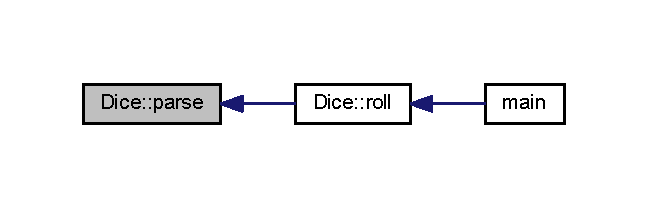
\includegraphics[width=311pt]{class_dice_a7fb1c52019fa79aa3b73e6610da9139c_a7fb1c52019fa79aa3b73e6610da9139c_icgraph}
\end{center}
\end{figure}
\hypertarget{class_dice_a4ca42849612d2c9182f1d93deaa4cfb1_a4ca42849612d2c9182f1d93deaa4cfb1}{}\label{class_dice_a4ca42849612d2c9182f1d93deaa4cfb1_a4ca42849612d2c9182f1d93deaa4cfb1} 
\index{Dice@{Dice}!roll@{roll}}
\index{roll@{roll}!Dice@{Dice}}
\subsubsection{\texorpdfstring{roll()}{roll()}}
{\footnotesize\ttfamily int Dice\+::roll (\begin{DoxyParamCaption}\item[{const string \&}]{Expr }\end{DoxyParamCaption})\hspace{0.3cm}{\ttfamily [static]}}

rolls x dy dice, adds up the values and optionally adds z to it, returns the result Expr\+: regular expression in the format xdy\mbox{[}+z\mbox{]} returns -\/1 if the regular expression was not in the correct format Below are the variables

parsing the xdy+ z expression provided

if it is not in the right format this is the output

for each dice

outputs a random number in the range 1-\/dice\+Kind and add it to the result

add the final addition to the resultHere is the call graph for this function\+:\nopagebreak
\begin{figure}[H]
\begin{center}
\leavevmode
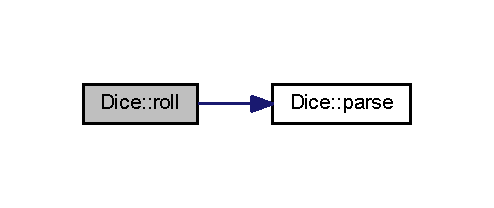
\includegraphics[width=237pt]{class_dice_a4ca42849612d2c9182f1d93deaa4cfb1_a4ca42849612d2c9182f1d93deaa4cfb1_cgraph}
\end{center}
\end{figure}
Here is the caller graph for this function\+:\nopagebreak
\begin{figure}[H]
\begin{center}
\leavevmode
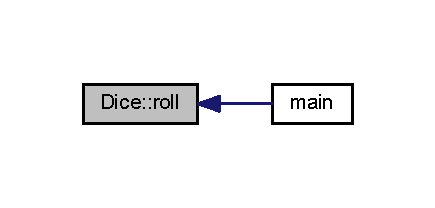
\includegraphics[width=209pt]{class_dice_a4ca42849612d2c9182f1d93deaa4cfb1_a4ca42849612d2c9182f1d93deaa4cfb1_icgraph}
\end{center}
\end{figure}


\subsection{Member Data Documentation}
\hypertarget{class_dice_afb857d94c4abede11939a308770ea72b_afb857d94c4abede11939a308770ea72b}{}\label{class_dice_afb857d94c4abede11939a308770ea72b_afb857d94c4abede11939a308770ea72b} 
\index{Dice@{Dice}!D\+I\+C\+E\+K\+I\+ND@{D\+I\+C\+E\+K\+I\+ND}}
\index{D\+I\+C\+E\+K\+I\+ND@{D\+I\+C\+E\+K\+I\+ND}!Dice@{Dice}}
\subsubsection{\texorpdfstring{D\+I\+C\+E\+K\+I\+ND}{DICEKIND}}
{\footnotesize\ttfamily const int Dice\+::\+D\+I\+C\+E\+K\+I\+ND = 7\hspace{0.3cm}{\ttfamily [static]}, {\ttfamily [private]}}

This indicates the number of different kinds of dice we have \hypertarget{class_dice_a0a00c7ba6e7486d9cbcf7c8c64c65b1a_a0a00c7ba6e7486d9cbcf7c8c64c65b1a}{}\label{class_dice_a0a00c7ba6e7486d9cbcf7c8c64c65b1a_a0a00c7ba6e7486d9cbcf7c8c64c65b1a} 
\index{Dice@{Dice}!D\+I\+C\+E\+N\+UM@{D\+I\+C\+E\+N\+UM}}
\index{D\+I\+C\+E\+N\+UM@{D\+I\+C\+E\+N\+UM}!Dice@{Dice}}
\subsubsection{\texorpdfstring{D\+I\+C\+E\+N\+UM}{DICENUM}}
{\footnotesize\ttfamily const int Dice\+::\+D\+I\+C\+E\+N\+UM = \{ 4, 6, 8, 10, 12, 20, 100 \}\hspace{0.3cm}{\ttfamily [static]}, {\ttfamily [private]}}

contains the y value for each dy dice 

The documentation for this class was generated from the following files\+:\begin{DoxyCompactItemize}
\item 
C\+:/\+Users/\+Asma Laaribi/\+Documents/\+Visual Studio 2015/\+Projects/\+Project1/\+Project1/\hyperlink{_dice_8h}{Dice.\+h}\item 
C\+:/\+Users/\+Asma Laaribi/\+Documents/\+Visual Studio 2015/\+Projects/\+Project1/\+Project1/\hyperlink{_dice_8cpp}{Dice.\+cpp}\end{DoxyCompactItemize}

\chapter{File Documentation}
\hypertarget{_dice_8cpp}{}\section{C\+:/\+Users/\+Asma Laaribi/\+Documents/\+Visual Studio 2015/\+Projects/\+Project1/\+Project1/\+Dice.cpp File Reference}
\label{_dice_8cpp}\index{C\+:/\+Users/\+Asma Laaribi/\+Documents/\+Visual Studio 2015/\+Projects/\+Project1/\+Project1/\+Dice.\+cpp@{C\+:/\+Users/\+Asma Laaribi/\+Documents/\+Visual Studio 2015/\+Projects/\+Project1/\+Project1/\+Dice.\+cpp}}
{\ttfamily \#include \char`\"{}Dice.\+h\char`\"{}}\newline
{\ttfamily \#include $<$stdlib.\+h$>$}\newline
{\ttfamily \#include $<$iostream$>$}\newline
{\ttfamily \#include $<$time.\+h$>$}\newline
Include dependency graph for Dice.\+cpp\+:\nopagebreak
\begin{figure}[H]
\begin{center}
\leavevmode
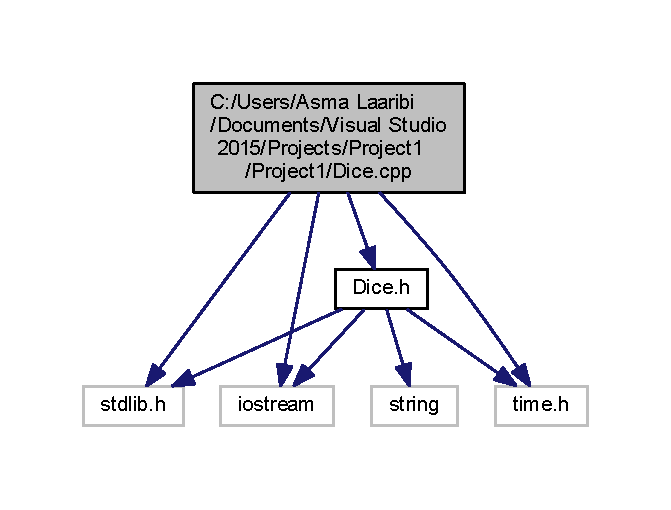
\includegraphics[width=322pt]{_dice_8cpp__incl}
\end{center}
\end{figure}

\hypertarget{_dice_8h}{}\section{C\+:/\+Users/\+Asma Laaribi/\+Documents/\+Visual Studio 2015/\+Projects/\+Project1/\+Project1/\+Dice.h File Reference}
\label{_dice_8h}\index{C\+:/\+Users/\+Asma Laaribi/\+Documents/\+Visual Studio 2015/\+Projects/\+Project1/\+Project1/\+Dice.\+h@{C\+:/\+Users/\+Asma Laaribi/\+Documents/\+Visual Studio 2015/\+Projects/\+Project1/\+Project1/\+Dice.\+h}}
{\ttfamily \#include $<$stdlib.\+h$>$}\newline
{\ttfamily \#include $<$iostream$>$}\newline
{\ttfamily \#include $<$time.\+h$>$}\newline
{\ttfamily \#include $<$string$>$}\newline
Include dependency graph for Dice.\+h\+:\nopagebreak
\begin{figure}[H]
\begin{center}
\leavevmode
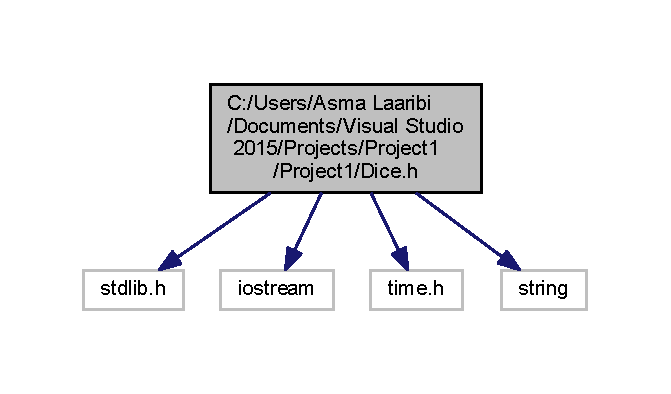
\includegraphics[width=322pt]{_dice_8h__incl}
\end{center}
\end{figure}
This graph shows which files directly or indirectly include this file\+:\nopagebreak
\begin{figure}[H]
\begin{center}
\leavevmode
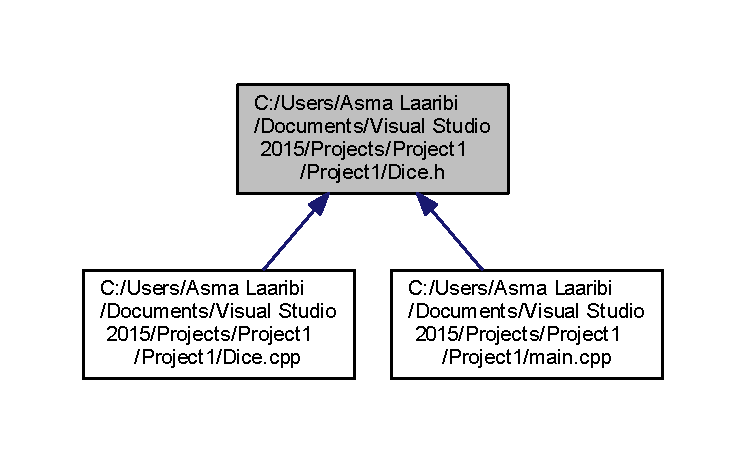
\includegraphics[width=350pt]{_dice_8h__dep__incl}
\end{center}
\end{figure}
\subsection*{Classes}
\begin{DoxyCompactItemize}
\item 
class \hyperlink{class_dice}{Dice}
\end{DoxyCompactItemize}

\hypertarget{main_8cpp}{}\section{C\+:/\+Users/\+Asma Laaribi/\+Documents/\+Visual Studio 2015/\+Projects/\+Project1/\+Project1/main.cpp File Reference}
\label{main_8cpp}\index{C\+:/\+Users/\+Asma Laaribi/\+Documents/\+Visual Studio 2015/\+Projects/\+Project1/\+Project1/main.\+cpp@{C\+:/\+Users/\+Asma Laaribi/\+Documents/\+Visual Studio 2015/\+Projects/\+Project1/\+Project1/main.\+cpp}}
{\ttfamily \#include \char`\"{}Dice.\+h\char`\"{}}\newline
{\ttfamily \#include $<$iostream$>$}\newline
Include dependency graph for main.\+cpp\+:\nopagebreak
\begin{figure}[H]
\begin{center}
\leavevmode
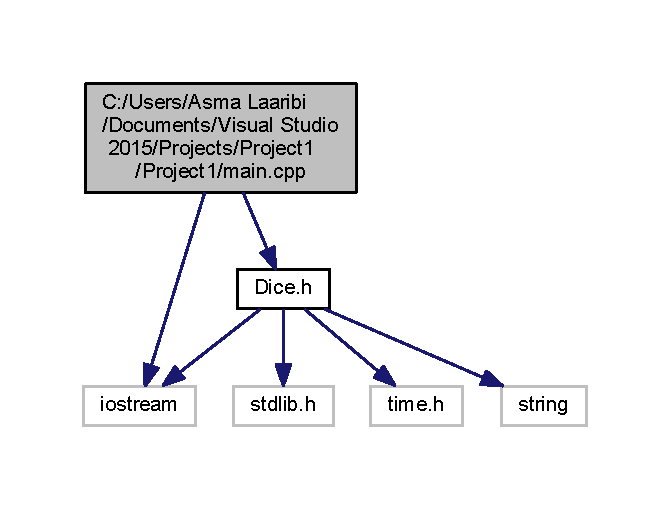
\includegraphics[width=322pt]{main_8cpp__incl}
\end{center}
\end{figure}
\subsection*{Functions}
\begin{DoxyCompactItemize}
\item 
int \hyperlink{main_8cpp_ae66f6b31b5ad750f1fe042a706a4e3d4_ae66f6b31b5ad750f1fe042a706a4e3d4}{main} ()
\end{DoxyCompactItemize}


\subsection{Function Documentation}
\hypertarget{main_8cpp_ae66f6b31b5ad750f1fe042a706a4e3d4_ae66f6b31b5ad750f1fe042a706a4e3d4}{}\label{main_8cpp_ae66f6b31b5ad750f1fe042a706a4e3d4_ae66f6b31b5ad750f1fe042a706a4e3d4} 
\index{main.\+cpp@{main.\+cpp}!main@{main}}
\index{main@{main}!main.\+cpp@{main.\+cpp}}
\subsubsection{\texorpdfstring{main()}{main()}}
{\footnotesize\ttfamily int main (\begin{DoxyParamCaption}{ }\end{DoxyParamCaption})}

Prompts the question to the user of how many dice they would like to roll

Then prompts the user to pick a kind of dice from the ones presented

Prompts if any additions would like to be added

provides the resultHere is the call graph for this function\+:\nopagebreak
\begin{figure}[H]
\begin{center}
\leavevmode
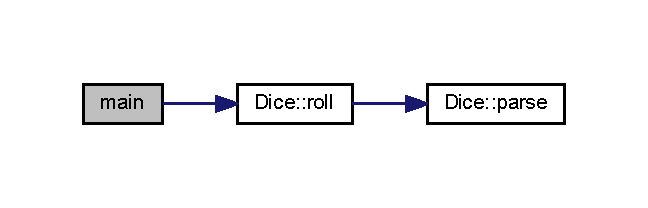
\includegraphics[width=311pt]{main_8cpp_ae66f6b31b5ad750f1fe042a706a4e3d4_ae66f6b31b5ad750f1fe042a706a4e3d4_cgraph}
\end{center}
\end{figure}

%--- End generated contents ---

% Index
\backmatter
\newpage
\phantomsection
\clearemptydoublepage
\addcontentsline{toc}{chapter}{Index}
\printindex

\end{document}
